
\section{Etica della donazione e dei trapianti}
 

\subsection{Le fonti normative: leggi e regolamenti}


Quella dei trapianti è una branca interdisciplinare, che riguarda non
solo i nefrologi, ma anche i chirurghi, gli immunologi, i laboratoristi,
coinvolgendo molte discipline e richiedendo grande capacità
organizzativa e di coordinamento, per quella che è sicuramente la
chirurgia di livello più elevato.
\\
Quali sono le fonti normative dei trapianti? Si parte con la
\textbf{legge 458 del 1967} che regola il trapianto di rene fra persone
viventi, per arrivare a una legge importante, la legge \textbf{644 del
1975}. Questa legge andava a regolarizzare il comportamento davanti a un
donatore di organo e indicava il tipo di attività, di controlli e di
esami che andavano fatti in un ipotetico donatore. Questa legge lasciava
però molti aspetti dell'attività scoperti.
\\
Un'altra legge importante è stata la \textbf{578 del '93}, che
codificava con più precisione la metodica di accertamento della morte
cerebrale, il grande problema che ancora oggi si ha con i cittadini, con
la società civile, che identifica la morte non con la mancata attività
cerebrale, ma con la cessazione dell'attività cardiaca.
\\
C'è poi stato il \textbf{decreto del '94} che istituiva per la prima
volta sul nostro territorio un Centro Nazionale di Riferimento (non
l'attuale) presso l'Istituto Superiore di Sanità e la Consulta Tecnica
dei trapianti, che era rappresentata da tutti i coordinatori regionali
dei Centri Regionali Trapianti di tutte le regioni. Si chiama CRT,
Centro Regionale Trapianti, ma non è un centro trapianti, un centro di
chirurgico, ma un centro di coordinamento, in passato chiamato Centro
Regionale di Riferimento per i Trapianti.
\\
La legge che ha poi dato la svolta nel campo trapiantologico, portando
l'Italia, da un penultimo posto in Europa davanti alla Grecia, ai primi
posti nel mondo per numero di trapianti, qualità e sicurezza degli
stessi, è la \textbf{legge 91 del '99}. Va ricordato che la sicurezza
dei trapianti è importante, avendo il trapianto grandi rischi anche per
comportamenti sbagliati da parte degli operatori, che possono causare la
morte del ricevente.
\\
La legge 91 ha una grande importanza perché per la prima volta in campo
nazionale anche i trapianti, e non solo l'AIDS o altre malattie
importanti, diventano obiettivi del servizio sanitario nazionale.
Secondo l'articolo 2, le Regioni e le Aziende Sanitarie, in
collaborazione con i CRT e i Centri Interregionali, devono adottare
tutte le misure per diffondere l'importanza del trapianto non solo tra i
cittadini, ma anche tra i medici e gli stessi rianimatori, dopo le
grandi difficoltà avute nel far capire quanto fosse importante
impegnarsi in un'attività di donazione. Con l'articolo 3 si entra in un
campo anche etico, dichiarando che all'inizio del periodo di
osservazione dell'ipotetico donatore ai fini dell'accertamento della
morte bisogna fornire informazioni sul prelievo di organi al coniuge non
separato o al convivente more uxorio o, in mancanza, ai figli maggiori
d'età o ai genitori. Questo è importante perché nel periodo iniziale non
si sapeva neanche chi fosse l'interlocutore del medico che andava a dire
ai familiari non solo che il figlio era morto, ma allo stesso tempo che
avrebbero voluto prelevarne gli organi. Questo è il momento più
difficile, per il quale abbiamo avuto come maestri gli Spagnoli, i primi
al mondo per attività di trapianto e capacità di organizzare corsi per
preparare i medici nel relazionarsi con i familiari, che è la cosa più
importante. Un prelievo diventa positivo solo se si ha la capacità di
saper parlare con il parente ed è una cosa difficile. In passato spesso
si contattavano i parenti nei corridoi, al volo, ed è la cosa più brutta
che si possa fare nei confronti di chi soffre per un familiare che sta
perdendo. Ora ci sono in quasi tutti gli ospedali stanze di accoglienza
dove si invitano i parenti a sedersi e si spiega cosa è la morte
cerebrale e qual è il fine di donare gli organi davanti a un bicchiere
d'acqua o un caffè. L'articolo 4 affronta il consenso. Ognuno può dare
il proprio consenso alla donazione, che può poi essere riportato sulla
carta d'identità. Se non si dà il proprio consenso né positivo né
negativo, si viene comunque considerati donatori. I soggetti a cui non
sia stata notificata la richiesta di manifestazione di volontà sono
considerati non donatori. Questo perché sarebbe dovuta arrivare ai
cittadini, secondo le disposizioni del ministro Bindi, una richiesta di
manifestazione di volontà, che però non è stata ricevuta da tutti. Però
quella del ``silenzio-assenso'' è una strategia che non è mai stata
applicata, perché ci sarebbe stata una guerra con i familiari che
avrebbe avuto l'effetto contrario, riducendo in realtà il numero di
prelievi di organo invece che aumentarlo.
\\
Con la legge 91 si istituisce, nel 1999, il Centro Nazionale Trapianti,
composto dal Direttore dell'Istituto Superiore di Sanità, da un
Direttore Generale, che dal '94 è il dottor Alessandro Nanni Costa, e da
un rappresentante per le tre Agenzie che costituivano la rete
trapiantologica nazionale. Nel '94 c'è stato anche un decreto per
regolare le modalità dell'accertamento della morte cerebrale,
ulteriormente aggiornato nel 2008.
\begin{figure}[!ht]
\centering
	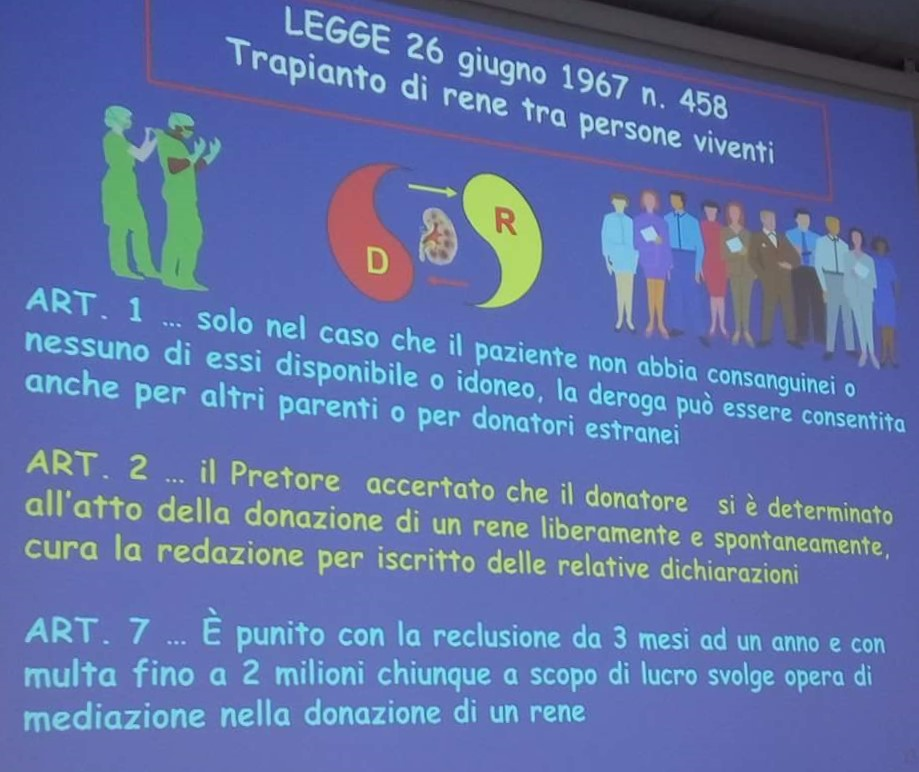
\includegraphics[width=0.7\textwidth]{34/image1.jpeg}
	\end{figure}


Tornando alla legge 458 del '67, essa disciplina il trapianto fra
donatori viventi, nello specifico quello di rene. I donatori viventi
sono rappresentati da familiari: coniugi, fratelli. Va preso in
considerazione l'aspetto del dono, perché ha un'implicazione per molti
versi terribile nei rapporti relazionali in famiglia.
\\
L'articolo 7 è stato abolito perché prevedeva la reclusione di tre mesi
più due milioni di lire di multa, mentre oggi sia la 91 che una legge
recente del 2015 presentata in Parlamento prevedono il carcere fino a 12
anni per chi fa commercio di organo, pubblicità o diffusione di questi
principi, e sospensione perpetua dalla pubblica amministrazione (e non
solo radiazione dall'Albo, che comunque non dura a vita, ma per un
periodo, alla fine del quale è possibile riscriversi).
\\
Il \textbf{decreto 116 del 2010} si occupa della donazione fra viventi
privi di legami di parentela, per assicurarsi che non ci siano dietro
alla donazione scopi di lucro o altri interessi. Molte volte chi dona
vorrebbe sapere chi è il ricevente. Per legge non è possibile dirlo,
perché può creare legami patologici fra donatore e ricevente. Non si
danno mai notizie sul ricevente, ma si informa la famiglia sul donatore
e si lascia a essa la libertà di decidere se entrare in contatto con
esso. Talvolta questo avviene e si instaura un rapporto positivo, altre
avviene e il rapporto instaurato non è totalmente positivo. Il medico
rimane comunque, per legge, al di fuori di queste dinamiche. La legge
del 2010, rispetto a quella del 1967, pone un'ulteriore terzietà nel
giudizio tramite una \emph{Commissione Terza}. Prima, il pretore
intervistava il possibile donatore per capire se fosse coinvolto
affettivamente e avesse corrette motivazioni o se alle spalle avesse
motivi di lucro, e dava il permesso per la donazione. Era coinvolto
anche uno psicologo che intervistava donatore e ricevente. Si è aggiunta
nel 2010 una Commissione Terza che non può essere composta dai chirurghi
dell'equipe, ma è rappresentata da terzi: coordinatori al trapianto,
psicologi... varie figure che possono assicurare che i riceventi e i
donatori potenziali abbiano agito secondo i principi del consenso
informato libero e consapevole e abbiano avuto tutte le informazioni del
caso sulla donazione e che altresì prevengono rischi di
commercializzazione di organi o di coercizione nella donazione, che può
avvenire anche in famiglia laddove un fratello debba dare un organo
all'altro fratello e intervengano i genitori.
\\
Il nostro Paese è tra i primi nel mondo per certificazione di qualità
nei trapianti e per l'attenzione che il trapianto sia fatto in strutture
appropriate. Il numero degli interventi crea la qualità, ma non si può
fare trapianto senza organi. Gli organi si ottengono solo se esiste un
efficace sistema di donazione. I trapianti però devono essere in numero
tale da assicurare la qualità e la sicurezza, senza scendere al di sotto
di un certo numero. Il CNT ha imposto delle regole, soprattutto per il
trapianto da vivente, oltre agli esami al donatore prima del prelievo.
Ad esempio, per il trapianto di fegato è necessario che la struttura
abbia effettuato, nell'anno solare precedente, almeno 25 trapianti da
cadavere. Si può iniziare un programma di trapianti da vivente
autorizzato dal Ministero della Salute e dall'Istituto Superiore di
Sanità solo se il centro ha all'attivo almeno 25 trapianti l'anno. Per
il rene, i trapianti da cadavere necessari sono 30. I livelli di qualità
devono poi essere paragonabili ai registri nazionali e internazionali
per quanto riguarda il follow-up e la sopravvivenza dell'organo
trapiantato.
\\
In Basilicata ci sono meno di 600mila abitanti e per quanto la Regione
possa raggiungere un numero di prelievi per milione di abitanti
paragonabili al dato nazionale, che è intorno ai 20-21 pmp, si
dovrebbero eseguire 10 prelievi. Questo non è un numero che permette di
avere l'autorizzazione a trapiantare, perché il centro non assicurerebbe
la qualità. Le liste sono regionali, quindi l'organo viene offerto prima
alle persone in lista nella regione e poi su tutto il territorio
nazionale, se non c'è compatibilità. L'organo e il paziente a cui viene
assegnato vengono mandati al Centro Trapianti del Policlinico La
Sapienza di Roma con cui la Basilicata ha un accordo di attività
chirurgica: il solo atto chirurgico viene fatto a Roma, mentre il
prelievo, l'assegnazione e il follow-up (terapia immunosoppressiva,
controllo delle complicazioni...) di tutta la regione vengono fatti in
Basilicata, per evitare i ``viaggi della speranza'' (che in passato
erano soprattutto all'estero) e uno spreco di soldi pubblici.
\\
Poi c'è stato il \textbf{Decreto del 2012}, che ricostituisce il CNT e
l'\textbf{Accordo Stato Regione del 2013} dove il CNT cambia aspetto
(non è più un centro di coordinamento ma diventa anche un centro
operativo), esiste un Centro Regionale ed esistono i Centri
Multiregionali.
\\
Queste sono leggi importanti sulla certificazione della morte cerebrale:
la \textbf{578 del '93} e la \textbf{582 del '94}. La 578 dà una
definizione giuridica della morte, stabilendo che ``\emph{la morte si
identifica con la cessazione irreversibile di tutte le funzioni
dell'encefalo}''. La 582 individua le modalità per l'accertamento e la
certificazione della morte. Questa legge poi è stata aggiornata nel
2008.

\begin{figure}[!ht]
\centering
	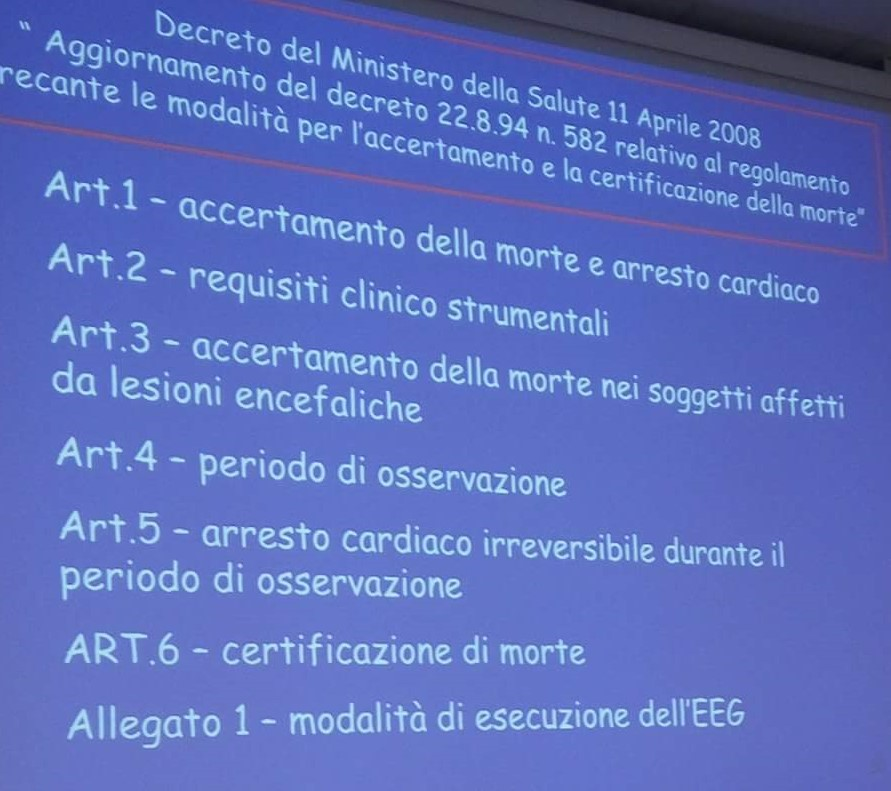
\includegraphics[width=0.7\textwidth]{34/image2.jpeg}
	\end{figure}

Se uno ha un insulto anossico non può essere sottoposto all'accertamento
di un EEG se non passano almeno 24 h dall'insulto stesso. Questo per far
sì che l'accertamento della morte sia assolutamente corretto, perché noi
con l'accertamento definiamo morto quell'individuo e andiamo a proporre
ai familiari l'espianto di organi. L'arresto cardiaco può avvenire
durante il periodo di osservazione; se avviene bisogna fare accertamento
della morte cardiaca e si fa con un ECG che deve durare 20 minuti. Che
accade però se va in arresto cardiaco un donatore a cui sto facendo
l'esame di morte cerebrale con EEG? Siccome l'arresto cardiaco avviene
in maniera istantanea, in ospedale, è possibile prelevare il rene (se
c'è un organo che può avere possibilità di ripresa, riperfondendolo una
volta prelevato, quello è il rene, per gli altri organi è difficile poi
trapiantarli). In alcune realtà sono stati fatti prelievi da donatore
con cuore fermo, con l'intento di aumentare il numero dei donatori (ad
esempio in Spagna hanno provato a fare prelievi sull'asfalto a pazienti
incidentati, ovviamente con tesserino di donatori).
\\
Poi viene descritta la modalità di esecuzione dell'EEG, che è complessa:
bisogna rispettare i microVolt, bisogna fare un tracciato che duri
mezz'ora di seguito per le 6h di osservazione, ci possono essere
problemi di bambini anencefalici su cui è difficile mettere gli
elettrodi.. Però c'è un'altra metodica che ci permette di dire che il
paziente è morto (se non posso eseguire un EEG) ed è quella del flusso
cerebrale (con un'angiografia posso dimostrare che non c'è flusso
ematico al cervello e quindi decretare la morte del paziente).
\\
\subsection{Il contesto: dati e organizzazione}


\subsubsection{Organizzazione in Italia fino al 2012}

\begin{figure}[!ht]
\centering
	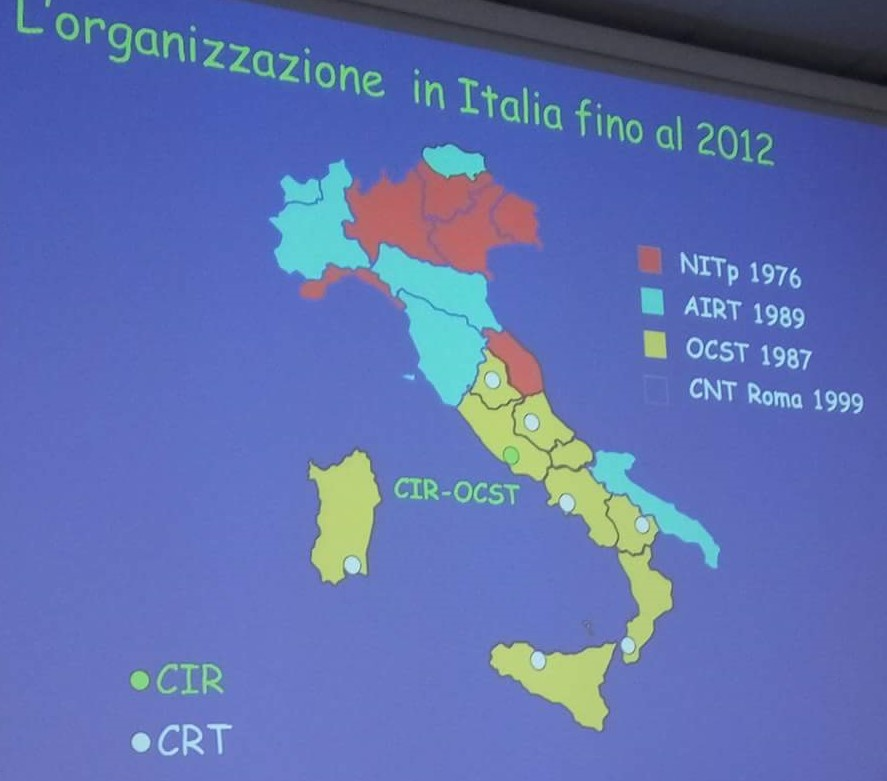
\includegraphics[width=0.7\textwidth]{34/image3.jpeg}
	\end{figure}

In Italia fino al 2012 c'era un Centro Nazionale a Roma istituito nel
1999 (CNT), poi c'erano 3 Agenzie, 3 raggruppamenti interregionali: NITp
(Nord Italia Transplant program), AIRT (Associazione InterRegionale
Trapianti) e OCST (Organizzazione Centro Sud Trapianti). Il CNT era
rappresentato dai 3 responsabili delle 3 Agenzie, dal Direttore Generale
e dal Direttore dell'Istituto Superiore di Sanità.

\begin{figure}[!ht]
\centering
	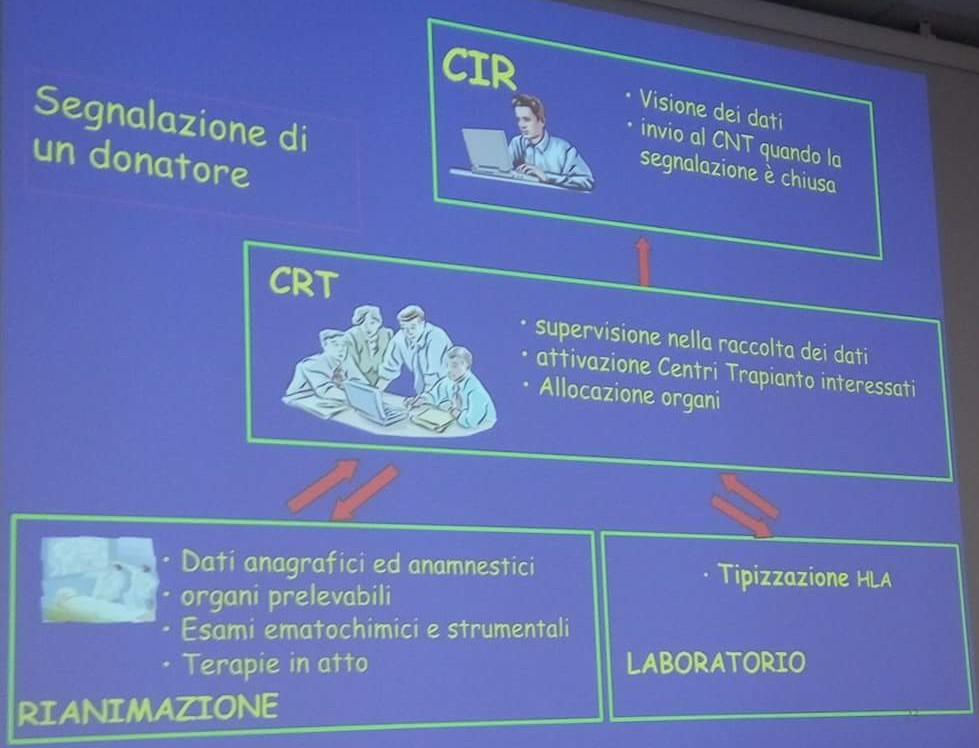
\includegraphics[width=0.7\textwidth]{34/image4.jpeg}
	\end{figure}

Questo è uno schema organizzativo della donazione d'organo. Il donatore
viene segnalato dalla rianimazione attraverso dati anagrafici e
anamnestici e dopo la valutazione degli organi prelevabili; viene
avvisato il Centro Regionale Trapianti (CRT). Questo centro raccoglie i
dati del paziente, gestisce la lista di tutti i pazienti in attesa di
trapianto, fa tutto ciò che è necessario, soprattutto la tipizzazione
HLA per la compatibilità tra donatore e ricevente. Tutto questo viene
osservato e valutato anche dal Centro InterRegionale (CIR) e
successivamente inviato al CNT. L'operatività quindi era del CRT e del
CIR; il CNT aveva un solo scopo: gestire le liste a carattere nazionale,
soprattutto la lista pediatrica, che non è mai stata regionale, ma
nazionale, per offrire ai bambini l'organo più compatibile per loro (non
su scala regionale ma nazionale).
\\
I principi di tutte le Agenzie erano principi di cooperazione, autonomia
e trasparenza; pur stando insieme, ogni regione rispettava una propria
autonomia nelle scelte, anche se ovviamente c'erano protocolli nazionali
comuni per quel che riguardava la gestione delle liste, i criteri di
assegnazione dell'organo (molto importanti da un punto di vista etico)
\ldots{} Se in un'Agenzia l'organo non trovava un paziente compatibile
esso veniva offerto alle altre due Agenzie, con obbligo di restituzione
(ovvero le altre due si impegnavano a restituirlo nel momento in cui ci
fosse stato un organo disponibile per i pazienti in lista d'attesa di
quella Agenzia).
\\
Poi c'era anche il registro dei cerebrolesi che aveva 3 funzioni:
archivio dei pazienti affetti da lesioni encefaliche, integrazione con
il sistema GEDON, ricerche e statistiche sui dati regionali.

\subsubsection{Organizzazione in Italia dopo il 2012}


\begin{figure}[!ht]
\centering
	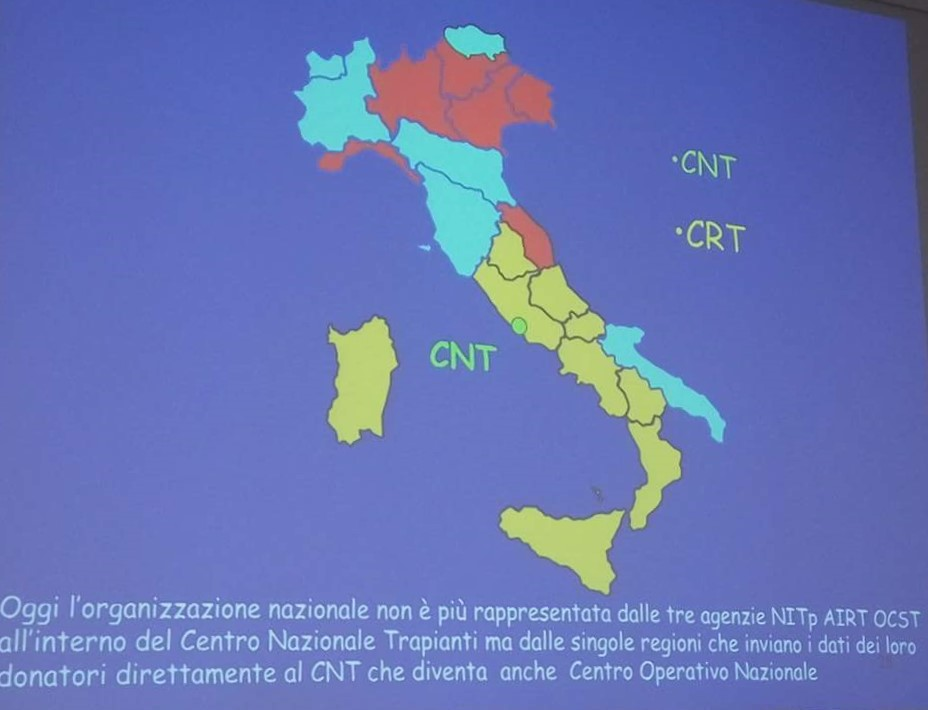
\includegraphics[width=0.7\textwidth]{34/image5.jpeg}
	\end{figure}

Oggi in Italia non c'è più il CIR, non esiste come attività di
coordinamento, ma se diverse Regioni vogliono mettersi insieme in un
Interregionale lo possono fare. Ora il CNT diventa operativo; mentre
prima l'operatività era in mano al CRT e al CIR ora è in mano al CRT e
al CNT. L'organizzazione e la metodologia rimangono uguali.

\begin{figure}[!ht]
\centering
	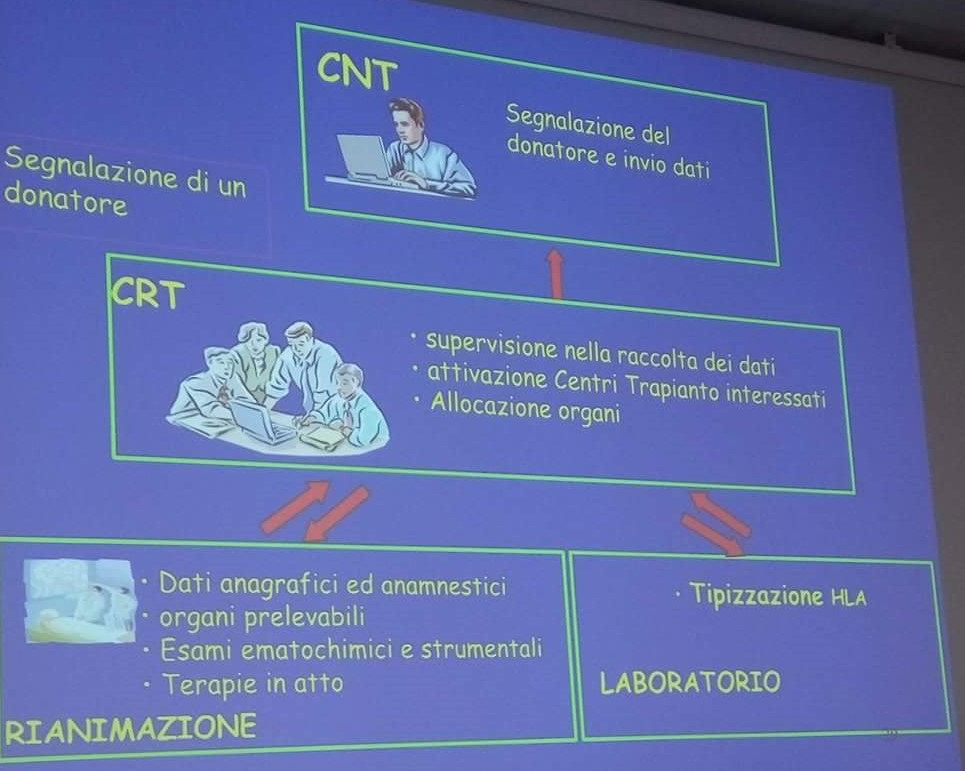
\includegraphics[width=0.7\textwidth]{34/image6.jpeg}
	\end{figure}

\subsubsection{Dati nazionali 2016}


8856 pazienti in lista d'attesa per trapianto, 1596 donatori totali e
1303 utilizzati (c'e stata la segnalazione di 1596 pazienti ma sono
risultati idonei alla donazione 1303); son stati fatti 3736 trapianti di
cui 319 da donatore vivente. I cittadini che hanno espresso la loro
volontà di donatori sono 1.852.767 di cui la maggior parte attraverso
l'AIDO, una quota minima invece attraverso le Asl e i Comuni. 16.518
persone hanno detto di no. Siccome la maggior parte della popolazione
italiana non ha espresso la propria volontà noi potremmo considerarli,
secondo la legge, donatori a tutti gli effetti.
\\
I tempi di attesa in lista sono notevolmente ridotti rispetto al
passato: per il rene ad esempio servono 3 anni, con una mortalità in
lista dell'1,6\%. Sono dati assolutamente di grande qualità e dimostrano
come l'attività trapiantologica del nostro Paese abbia avuto
un'evoluzione nettamente positiva.

\begin{figure}[!ht]
\centering
	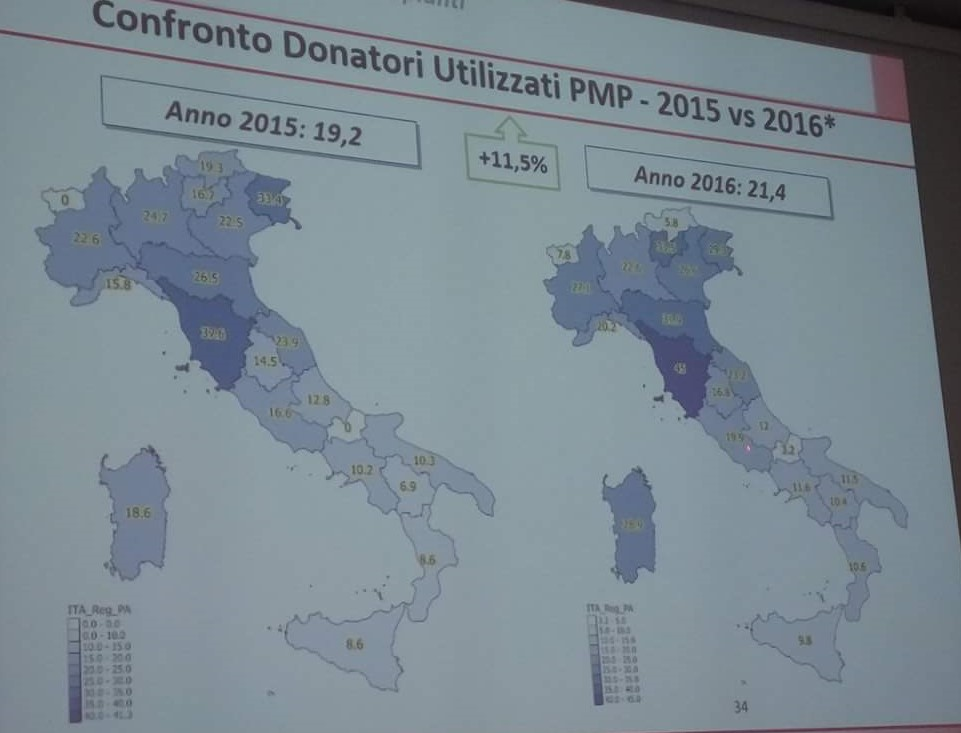
\includegraphics[width=0.7\textwidth]{34/image7.jpeg}
	\end{figure}

Questi sono dati di raffronto tra 2015 e 2016: c'è stato un incremento
nel 2016 sia del numero delle donazioni sia del numero di trapianti
effettuati. Per quanto riguarda l'attività di donazione, le Regioni del
Sud soffrono notevolmente (la Sicilia fa 9.8 pmp mentre la Toscana fa 45
pmp) e la differenza Nord-Sud è ancora un problema da risolvere (i
motivi sono vari, culturali, di migrazione di giovani ecc..). Le regioni
leader sono la Toscana, l'Emilia Romagna e il Friuli Venezia Giulia.
\\
Un dato fondamentale su cui riflettere è questo: quante persone ci hanno
detto di no nel momento in cui abbiamo proposto di espiantare gli
organi? Le percentuali sono alte: la Basilicata è al 52\%, la Calabria
al 44\%, l'Abruzzo al 41\%, mentre nelle Regioni del Nord l'opposizione
ai trapianti ha una media più bassa. Una Regione a parte è la Sardegna,
sia per numero di trapianti che per numero di prelievi. Qual è il motivo
dell'opposizione? Siamo poco bravi ad affrontare il rapporto con i
familiari? Non abbiamo lavorato in modo sufficiente per implementare la
cultura dei medici e dei cittadini nel settore trapianto logico?

\subsubsection{Chi può donare gli organi}


\emph{Donatore cadavere}: ogni soggetto in cui sia stata fatta diagnosi
di morte viene considerato donatore d'organo, senza alcuna differenza
d'età. Vi sono delle eccezioni per soggetti con alcune patologie (vedi
dopo). Poi viene fatta la valutazione del donatore e si valutano le
condizioni dell'organo (se è trapiantabile e con quale possibilità di
sopravvivenza a distanza). Nel caso di organi di pazienti anziani si può
fare il trapianto doppio: si possono prelevare entrambi i reni e
trapiantarli tutti e due nello stesso soggetto per avere una
funzionalità sommata. Nel caso del fegato a Torino c'è un centro che
preleva l'organo da persone anche anziane (\textgreater{}80 anni),
ovviamente il ricevente deve essere selezionato in base a vari criteri,
non ultimo quello dell'età (non andrò mai a dare un fegato di un
ottantenne a un ragazzo di 20 anni).
\\
Le \emph{controindicazioni assolute} alla donazione sono: HIV*,
neoplasie maligne, malattia da prioni e infezioni sistemiche (ad esempio
TBC disseminata). * I donatori di organi HIV positivi possono donare ad
altri pazienti HIV positivi o anche a persone sieronegative ma in
pericolo estremo di vita per mancanza di altro organo compatibile (casi
rari ma comunque presenti), ovviamente con consenso informato.
\\
\emph{Donatore vivente}: rene e oggi anche fegato

\begin{figure}[!ht]
\centering
	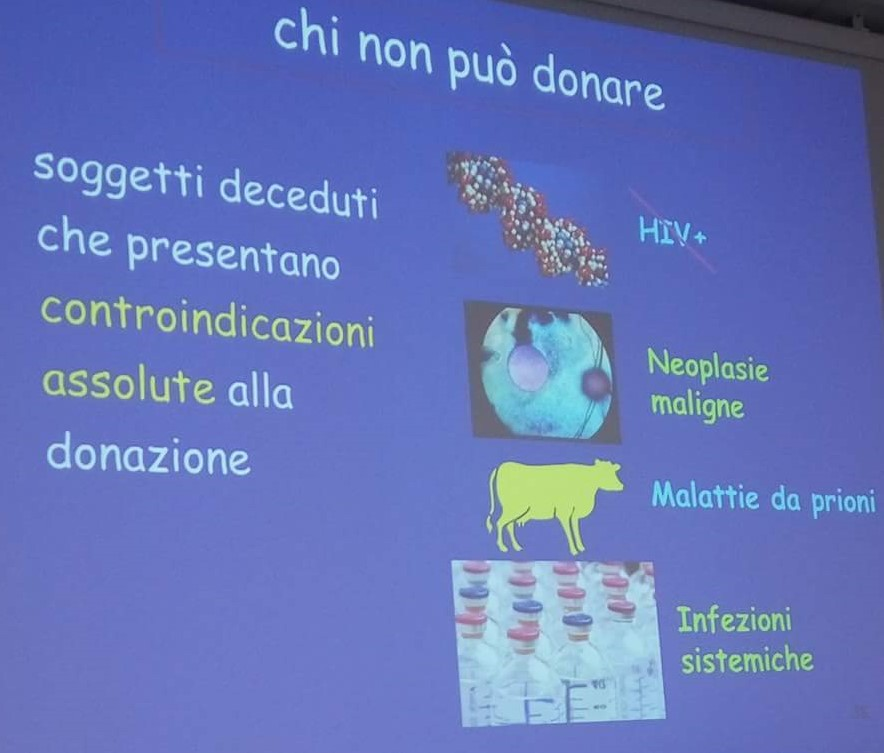
\includegraphics[width=0.7\textwidth]{34/image8.jpeg}
	\end{figure}

\subsection{Il codice deontologico}


\textbf{Art. 40}:'' \emph{il medico promuove la cultura della donazione
di organi, tessuti e cellule collaborando all'informazione dei cittadini
e sostenendo donatori e riceventi.} ``
\\
Non è una cosa scontata! L'importanza del MMG nell'applicare questo
articolo è estrema, ma il comportamento di molti colleghi purtroppo non
va sempre in questa direzione.
\\
\textbf{Art. 41}: ``\emph{Il prelievo da cadavere di organi, tessuti e
cellule a scopo di trapianto terapeutico è praticato nel rispetto
dell'Ordinamento garantendo la corretta informazione dei familiari. Il
prelievo da vivente è aggiuntivo e non sostitutivo del prelievo da
cadavere e il medico, nell'acquisizione del consenso informato scritto,
si adopera per la piena comprensione dei rischi da parte del donatore e
del ricevente}''. Questo vuol dire che non bisogna abbandonare il
programma e l'impegno a cercare un donatore cadavere perché tanto c'è un
familiare (anche se devo dire che da noi il trapianto da vivente non ha
ancora avuto quell'espansione che vediamo in altri Paesi)
\\
``\emph{Il medico non partecipa ad attività di trapianto nelle quali la
disponibilità di organi, tessuti e cellule abbia fini di lucro}''.
Questo potrebbe essere un motivo per finire in commissione disciplinare:
la legge punisce chiunque si macchi di questo delitto con l'esclusione
da qualunque incarico pubblico.
\\
\textbf{Art. 38}: \emph{Dichiarazioni anticipate di trattamento}. È la
storia dell'eutanasia, del destino che ognuno vorrebbe decidere da vivo
(ad esempio quali interventi terapeutici ricevere) per quando non avrà
più le capacità intellettive. È l'autodeterminazione della propria
persona. Sono argomenti molto delicati, soprattutto in un Paese che
ospita il Vaticano. La disponibilità a donare gli organi è una
dichiarazione anticipata di trattamento.

\begin{figure}[!ht]
\centering
	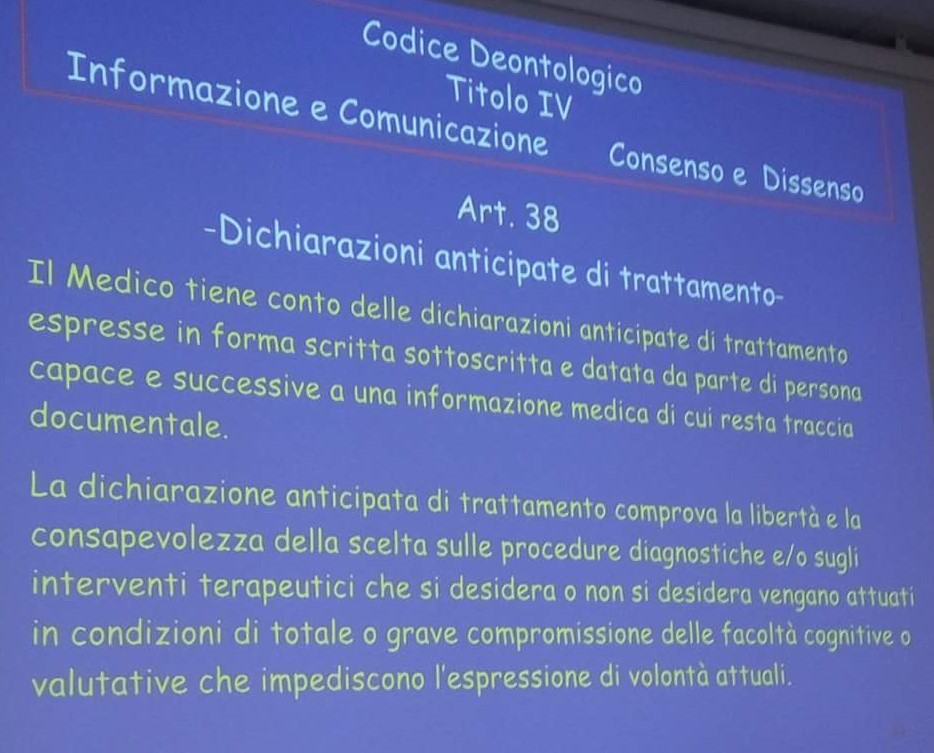
\includegraphics[width=0.7\textwidth]{34/image9.jpeg}
	\end{figure}
\subsection{L'etica}


\emph{``L'etica non è uno studio puramente accademico, senza alcuna
connessione con la vita quotidiana, ma chiunque sia costretto a
riflettere e sia turbato da certe situazioni è un filosofo morale''}
\\
Il medico dovrà risolvere ogni problema scegliendo la miglior linea di
condotta tecnico-morale possibile.

\begin{figure}[!ht]
\centering
	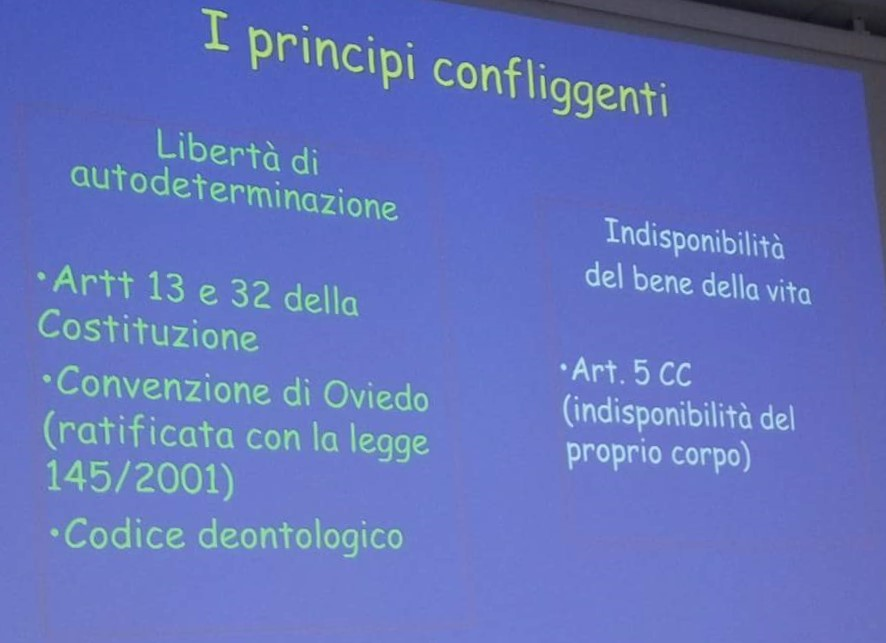
\includegraphics[width=0.7\textwidth]{34/image10.jpeg}
	\end{figure}

Quali sono i principi configgenti? Da una parte abbiamo la Costituzione
e la Convenzione di Oviedo che danno la libertà all'autodeterminazione,
dall'altra c'è il Codice Civile che pone l'indisponibilità del proprio
corpo. L'articolo 13 dice che la libertà personale è inviolabile,
l'articolo 32 che nessun soggetto può essere obbligato a un determinato
trattamento se non per disposizione di legge (TSO per malattie
psichiatriche) mentre il Codice Civile dice che gli atti di disposizione
del proprio corpo sono vietati quando cagionano un danno permanente
all'indennità fisica o quando siano contrari alla legge.
\\
Esistono quindi dei dilemmi etici:

\begin{enumerate}
\def\labelenumi{\arabic{enumi})}
\item
  È possibile conciliare l'autodeterminazione riconosciuta per legge al
  cittadino con la libertà del medico di decidere?
\item
  È utile che il medico sia un esecutore passivo delle volontà del
  malato come pretenderebbe qualcuno?
\end{enumerate}

A questo proposito vi faccio due esempi che sono stati la vergogna del
nostro sistema sanitario e della scienza medica in questo Paese: il caso
Di Bella e Stamina. Il caso Di Bella l'ho vissuto in prima persona come
amministratore in quanto ho dovuto rimborsare soldi a pazienti che
avevano deciso inutilmente di affidarsi al metodo Di Bella. Se la
volontà del malato è quella di andare da Di Bella son fatti suoi, ma io
non devo essere costretto a sostenere questo e a sottrarre risorse
economiche agli altri cittadini. Noi abbiamo un grave problema: il
contrasto tra la scienza e il diritto. Un magistrato non può arrogarsi
il diritto di decidere al nostro posto cosa è utile per il paziente, non
avendo egli alcuna base scientifica per decidere una cosa del genere. E
io da un Procuratore ho avuto l'imposizione di pagare praticamente una
terapia di cui non condividevo non l'utilità. Stessa cosa per Stamina.
Come si può permettere uno che non è nemmeno un medico di decidere in un
ambito in cui non ha nessuna conoscenza, sfruttando la speranza e la
malattia dei pazienti? Perché alla fine chi ha una malattia grave si
aggrappa a tutto, anche alla vitamina A di Di Bella. Questo è quello che
abbiamo dovuto subire con Di Bella. Ho sottratto soldi che avrei potuto
utilizzare per chi ha realmente bisogno. Se noi evitassimo di fare tanti
esami inutili potremmo avere le risorse per dare tutto a tutti.
\\
Noi siamo passati da un periodo in cui ci veniva perdonato tutto ad
oggi, in cui il cittadino ha avuto un'evoluzione da paziente a cliente a
utente a cibernauta (il cittadino apre internet e viene dal medico in
una situazione di totale informazione ed è esigente e spesso è anche
conflittuale nei rapporti). Noi dobbiamo andare a recuperare il rapporto
perso con i pazienti. Se voi andate dal sarto e decidete di prendere un
vestito che vi piace, preferireste un vestito industriale o sartoriale?
Sicuramente quello sartoriale. Lo stesso fa il paziente, il paziente
vuole una medicina che sia sartoriale ossia una medicina che sia basata
sulla sua individualità e che non sia uguale per tutti. Questo rapporto
medico-paziente noi lo abbiamo perso negli anni, a seguito al processo
di aziendalizzazione (ad esempio se si richiede al cardiologo di fare 40
visite l'ora perché si deve fare un tot. di DRG, si perde qualunque tipo
di rapporto con il paziente). Noi abbiamo perso, in tutti questi anni,
il rapporto relazionale con il paziente perché non abbiamo più il tempo
di parlare e di ascoltare. Questo ha abbassato il livello qualitativo .
\\
La soluzione dell'accanimento terapeutico noi lo abbiamo risolto nei
trapianti con la 578. Se non avessimo avuto questa legge noi non avremmo
potuto fare l'accertamento della morte, e quindi che cosa non avremmo
potuto fare? Non avremmo potuto smettere una terapia inutile, perché nel
momento in cui il paziente viene definito in morte cerebrale, qualunque
tipo di terapia è inutile, il paziente è destinato a morire (perché se
noi stacchiamo il respiratore, stacchiamo le funzioni che manteniamo in
modo artificiale, il paziente è morto). Se non avessimo avuto questa
legge non avremmo potuto fare né il prelievo ma soprattutto non avremmo
potuto evitare l'accanimento terapeutico. Ora si tengono in piedi
ospedali che non sono tali, sono sì e no poliambulatori, ma il cittadino
li considera veri e propri ospedali, entra e poi non può ricevere le
cure che un ospedale dovrebbe dare. In questi ospedali spesso ci sono
pseudo-rianimazioni. Una delle regole fondamentali perché una struttura
possa essere definita rianimazione è che sappia fare questo: se un
ospedale non è in grado di fare accertamento della morte (e per farlo
c'è bisogno di personale specializzato) non dovrebbe nemmeno aprire, non
solo per il prelievo degli organi, ma anche perché l'accertamento della
morte mi permette di restituire il paziente ai parenti e al contempo di
liberare un posto in rianimazione ed evitare che una persona con trauma
cranico muoia in giro per ospedali mentre cerca un posto libera in
terapia intensiva (purtroppo è una cosa che accade ogni giorno). Questa
legge ci ha permesso di rendere più etico il nostro SSN, ma non si può
fare ovunque perché l'ospedale per fare questo deve avere questa
attività.
\begin{figure}[!ht]
\centering
	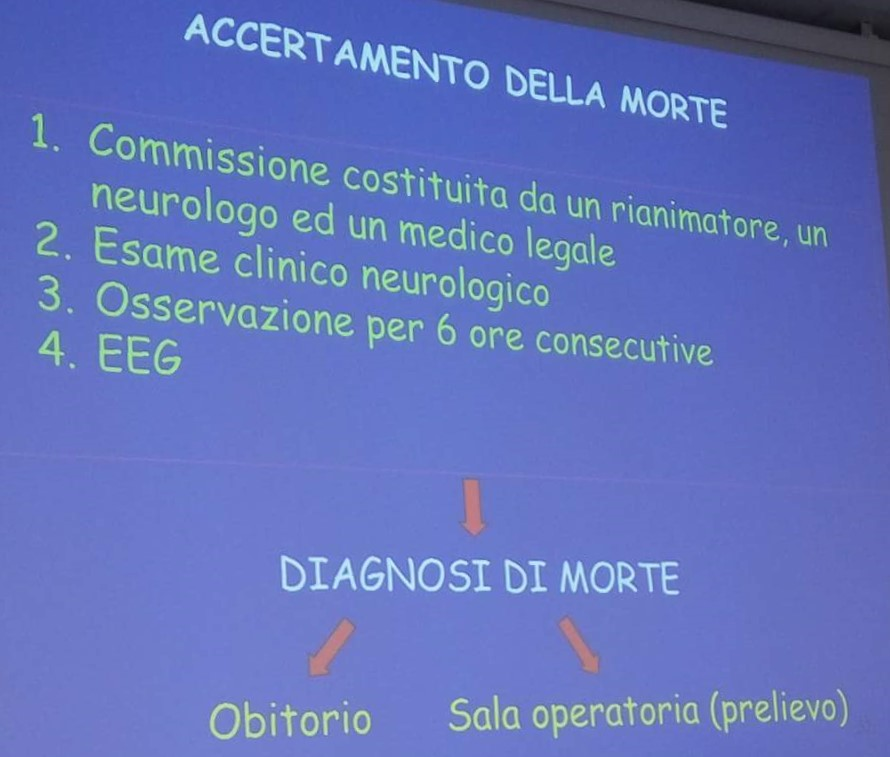
\includegraphics[width=0.7\textwidth]{34/image11.jpeg}
	\end{figure}

C'è bisogno di una commissione che abbia un rianimatore, un neurologo
esperto in EEG e un medico legale, deve essere fatto un esame clinico
neurologico, un EEG e il paziente deve essere messo in osservazione per
6 h consecutive. Allora, fatta la diagnosi di morte, indipendentemente
dal fatto che possa o meno essere donatore, o va in obitorio o va in
sala operatoria per il prelievo.
\\
Se ho un donatore in un ospedale che non può fare accertamento di morte,
potremmo anche prendere il paziente e trasferirlo, però dobbiamo pensare
alla famiglia: dovrebbe seguire il proprio caro, per lunghe distanze, e
questo è eticamente scorretto. Ecco perché una rianimazione che non ha
tutti i parametri necessari per fare attività rianimatoria e
accertamento di morte non dovrebbe nemmeno aprire.

\begin{figure}[!ht]
\centering
	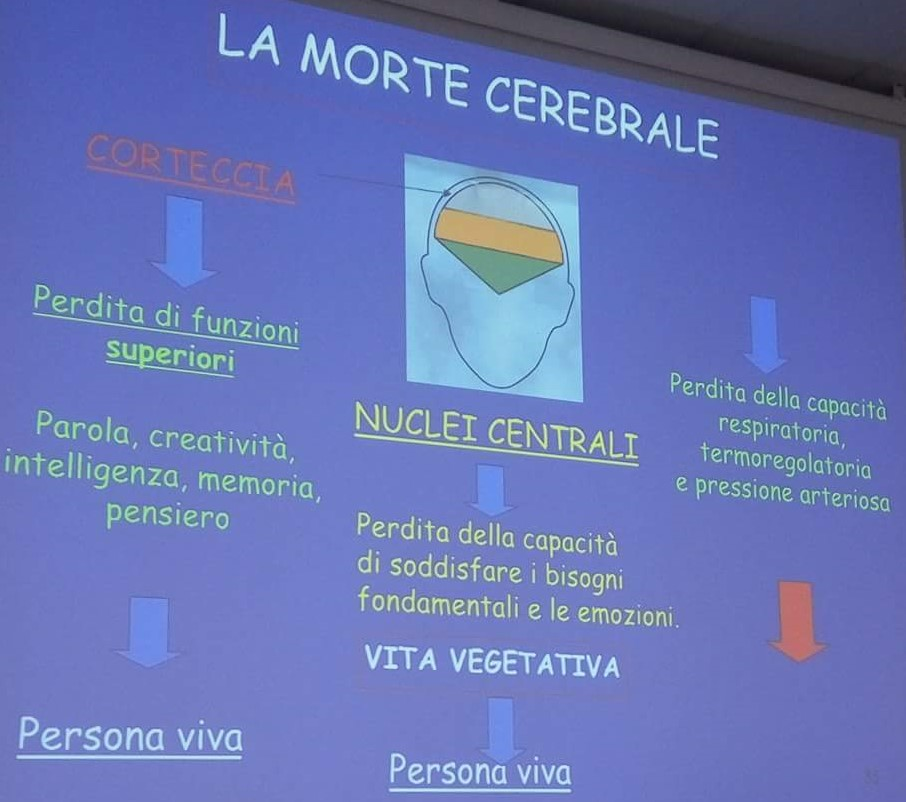
\includegraphics[width=0.7\textwidth]{34/image12.jpeg}
	\end{figure}

La morte cerebrale provoca arresto dell'attività cardiaca e arresto
dell'attività respiratoria, funzioni che noi manteniamo artificialmente.
Esiste una sola morte cerebrale? Possiamo avere lesioni della corteccia
che determinano la perdita di funzioni superiori quali parola,
creatività, intelligenza, memoria ma la persona è viva. Ci può essere un
danno ai nuclei centrali e quindi il paziente è in stato vegetativo;
infine ci può essere una lesione del tronco con perdita della capacità
respiratoria e in questo caso il paziente è morto. Ecco perché noi non
parliamo più di coma (che potremmo avere per lesioni della corteccia) ma
parliamo solo di morte cerebrale.
\\
Alcuni cittadini hanno dato il proprio consenso alla donazione, altri lo
hanno negato. Per la maggior parte dei cittadini questo dato manca. Per
la legge 91 dovremmo considerarli donatori, ma non lo facciamo e non lo
abbiamo mai fatto. A questo punto chiediamo ai familiari, andando però a
ledere il principio dell'autodeterminazione del soggetto. Ci sono le
stanze dell'accoglienza e andiamo direttamente dalla persona che ha, dal
punto di vista giuridico, il diritto di esprimere un parere (molto
spesso ci si trova con numerosi familiari e pareri contrastanti).
\\
Anche il Comitato Nazionale di bioetica dice che la decisione di
interrompere i trattamenti medici non proporzionati e privi di alcuna
credibile prospettiva terapeutica per il paziente è non solo lecita, ma
addirittura doverosa, per impedire che l'azione medica si trasformi in
accanimento terapeutico. È chiaro che tutto questo non deve creare
l'abbandono terapeutico.
\\
Non ci sono e non ci possono essere criteri per stabilire, dei nostri
mezzi terapeutici, quale sia ordinario e quale straordinario. I criteri
di definizione variano secondo le epoche storiche e i relativi contesti
socio-culturali. Non è neanche ben definito quale sia il ruolo del
paziente interessato dai nostri mezzi terapeutici. Nel contesto
socio-culturale attuale gli eventi del nascere e del morire erano
considerati dai nostri genitori eventi naturali, mentre oggi sono eventi
aperti al campo delle scelte private, all'autodeterminazione e ai
diritti di ciascun cittadino.
\\
Questo comporta che il paziente diventi protagonista del proprio congedo
dal mondo. Il problema consiste nel fatto che è il concetto di vita
umana ad essere incerto. Vi è una differenza significativa tra la vita
biologica e la vita biografica, cioè fra la vita e l'esistenza, e si va
sempre più affermando una concezione diversa del rapporto fra
l'individuo e il proprio corpo che diventa oggetto di volontà
individuale oltre che collettiva. Il diritto di disporre del proprio
corpo integrato dal principio di autodeterminazione, rientra nelle
nostre libertà individuali.
\\
L'attuale prassi applicata sulla donazione (consenso dei familiari in
caso di mancata espressione di volontà) entra in conflitto con il
principio dell'autodeterminazione. Non sappiamo quale sia la volontà
espressa dal soggetto, quindi ci rivolgiamo ai parenti, non rispettando
l'autodeterminazione dell'individuo. E la stessa conflittualità può
essere rilevata nel ``silenzio-assenso'', perché non rispetteremmo la
volontà, anche se non espressa, del cittadino. È necessario che sia i
medici che i politici inizino a ragionare su questi aspetti e a cercare
di migliorare le parti legislative. Ad ogni cittadino deve essere
consentito di compiere le proprie scelte etiche sulla propria vita,
definendone il senso, il significato, i limiti. Allo Stato rimane il
compito di assicurare le condizioni in cui tali scelte possono diventare
effettive.
\\
Tipologie di trapianto: \emph{autotrapianto}, \emph{omotrapianto} e
\emph{xenotrapianto}. C'è stato un lungo periodo in cui si sono fatte
ricerche, in centri universitari, sui maiali, considerando i loro organi
come i più affini e con più possibilità di dare un buon esito al
trapianto. Il solo problema sono i retrovirus, cioè la possibilità di
trasferire malattie dall'animale all'uomo, perché questo è un campo
ancora molto sperimentale e lasciato soltanto alla ricerca.
\\
Problematiche: definizione di morte (dalla morte cardiaca a quella
cerebrale), espressione e validità del consenso, quali organi
trapiantare e allocazione degli organi. Le varie tipologie di morte.
\\
Quali sono i problemi etici? La nuova definizione di morte (vale solo
per la persona umana ma non per altri mammiferi, e potrebbe essere
un'eccezione non giustificata sul piano biologico), la controintuitività
della morte cerebrale. Per noi è molto più intuitivo che una persona
muoia se ha un arresto cardiaco, è controintuitivo pensare che una
persona sia morta se ha avuto una lesione del tronco encefalico. La
nuova definizione di morte cerebrale non risolve i problemi per cui era
stata pensata, cioè la liceità del trapianto di organi. E sul piano
prescrittivo, al fine della liceità del prelievo di organi può essere
riconosciuta una nuova eccezione al principio di ``non uccidere'' quando
un individuo è entrato nel processo del morire e ha superato la soglia
di non ritorno. In questo caso, con il suo consenso libero e consapevole
precedentemente espresso, può essere lecito anticipare la morte. Questo
è un modo filosofico, etico, per definire la libertà di scelta di un
individuo e la morte cerebrale.

\begin{figure}[!ht]
\centering
	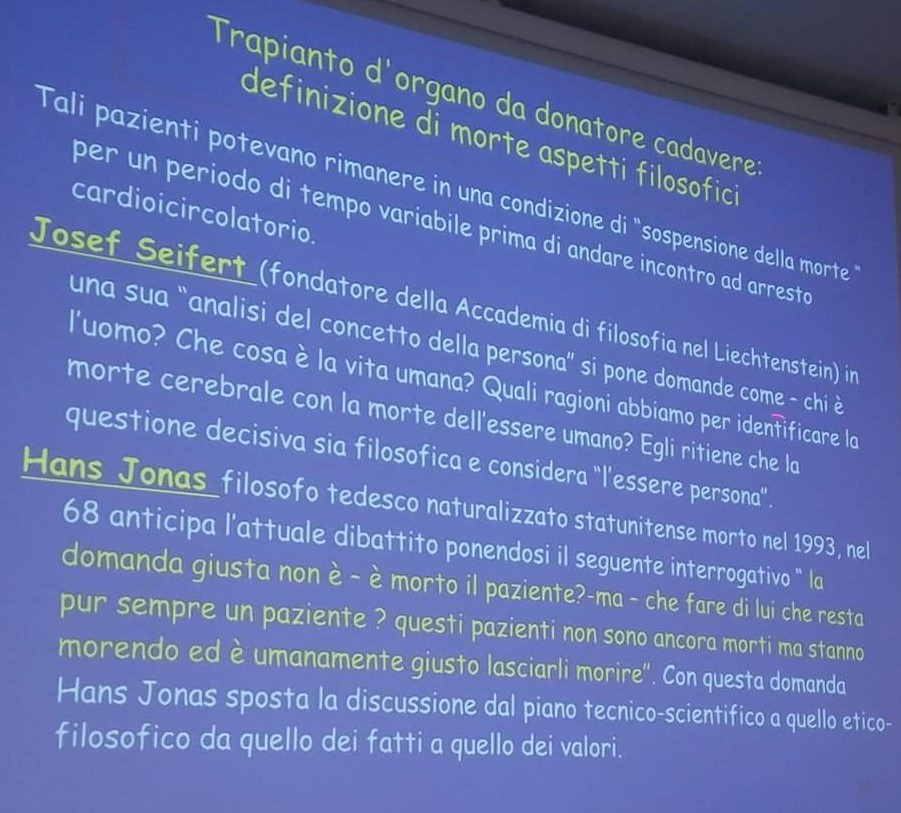
\includegraphics[width=0.7\textwidth]{34/image13.jpeg}
	\end{figure}

Alcuni filosofi non condividono (ma non è scienza) la definizione di
morte cerebrale.
\\
D. Lamb, autore di ``Etica e trapianto'', fa un paragone fra la morte
cerebrale nelle varie confessioni religiose

\begin{figure}[!ht]
\centering
	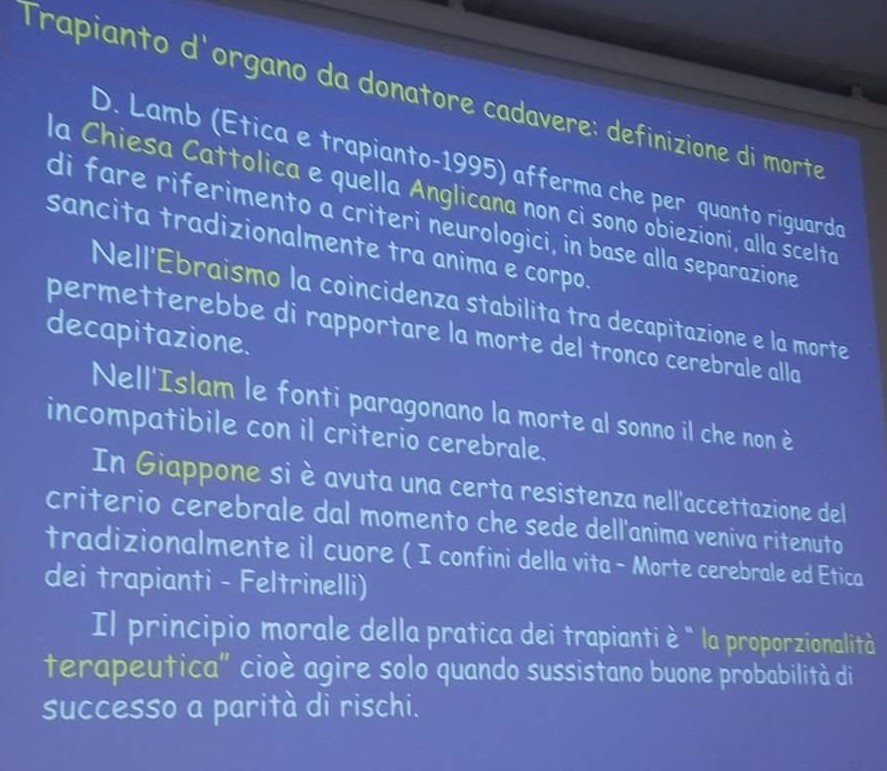
\includegraphics[width=0.7\textwidth]{34/image14.jpeg}
	\end{figure}

Al di là di tutto questo, il principio morale della pratica dei
trapianti è la ``proporzionalità terapeutica'', cioè si deve agire
quando si hanno buone probabilità di successo a parità di rischio, per
non agire in modo eticamente scorretto.
\\
Il consenso: il consenso dato dai familiari, il consenso dato dai
donatori (problema delle direttive anticipate), il problema del
``silenzio-assenso''.
\\
Chi necessita di un organo per sopravvivere può avanzare un diritto, una
pretesa ad averlo? Questa non è filosofia, abbiamo degli esempi pratici.
In India c'era un'associazione anglo-indiana che dava un milione di lire
al cittadino indiano che donava l'organo e il cittadino italiano pagava
sessanta milioni per averlo, fare il trapianto e tornare a casa. Questa
scelta, in passato, è stata fatta da alcuni cittadini che non volevano
aspettare. Tornando, però, pretendevano di avere il rimborso dei soldi,
cosa non corretta.
\\
Come si allocano gli organi? Ci sono vari criteri di allocazione.
\begin{figure}[!ht]
\centering
	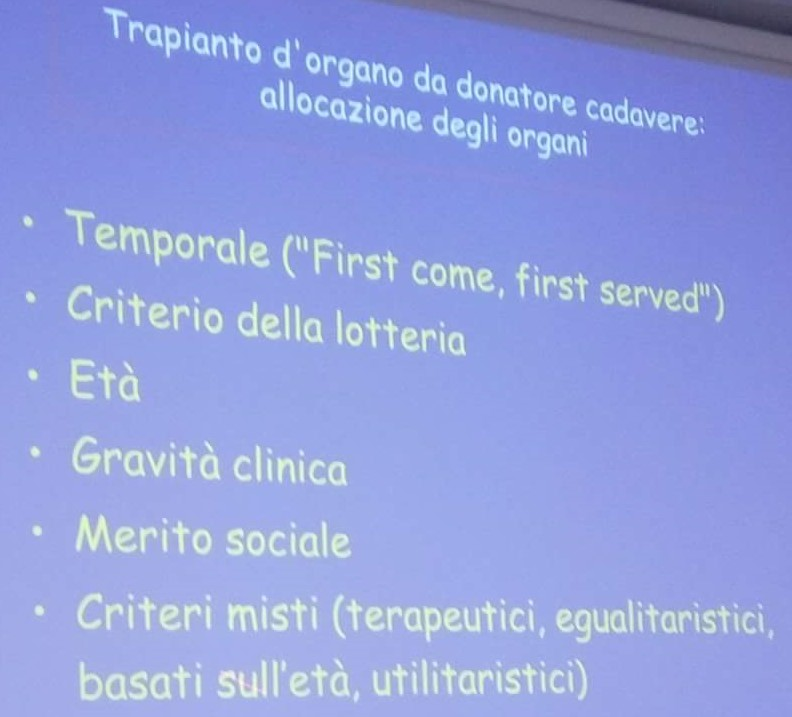
\includegraphics[width=0.7\textwidth]{34/image15.jpeg}
	\end{figure}

Quando tutto viene fatto in modo informatico non c'è possibilità di fare
favori a nessuno.
\begin{figure}[!ht]
\centering
	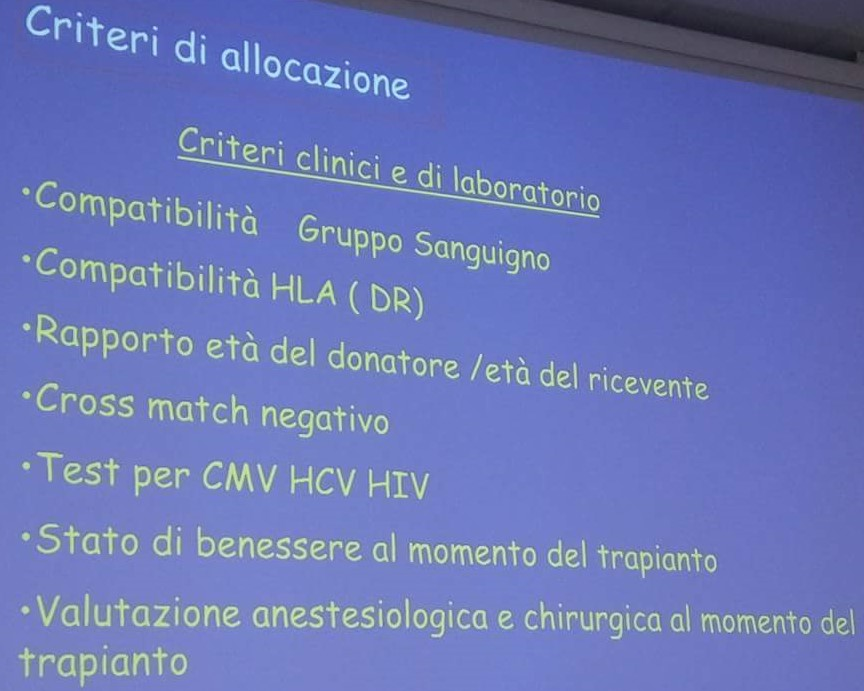
\includegraphics[width=0.7\textwidth]{34/image16.jpeg}
	\end{figure}

Il dono è il fondamento dei trapianti d'organo.

\begin{figure}[!ht]
\centering
	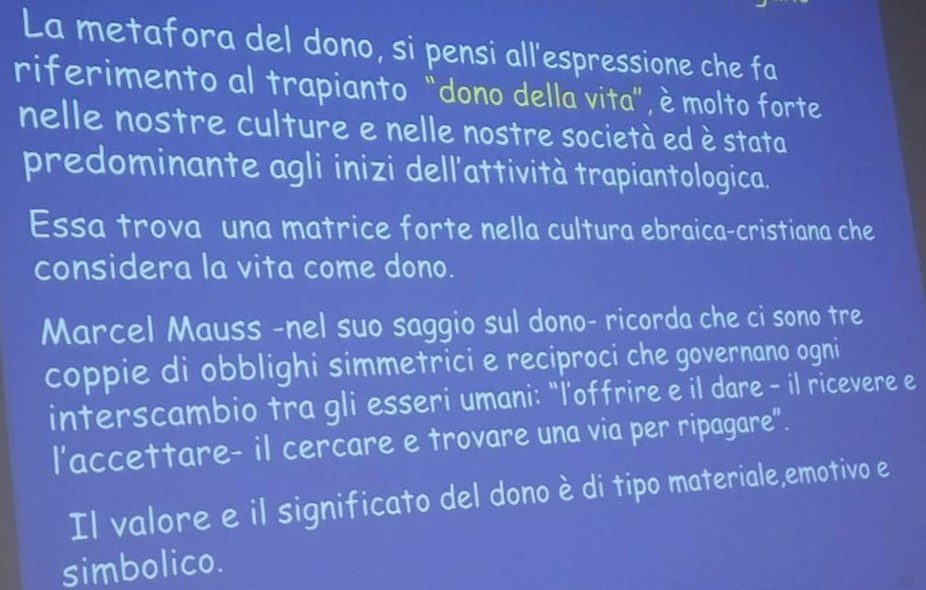
\includegraphics[width=0.7\textwidth]{34/image17.jpeg}
	\end{figure}

\begin{figure}[!ht]
\centering
	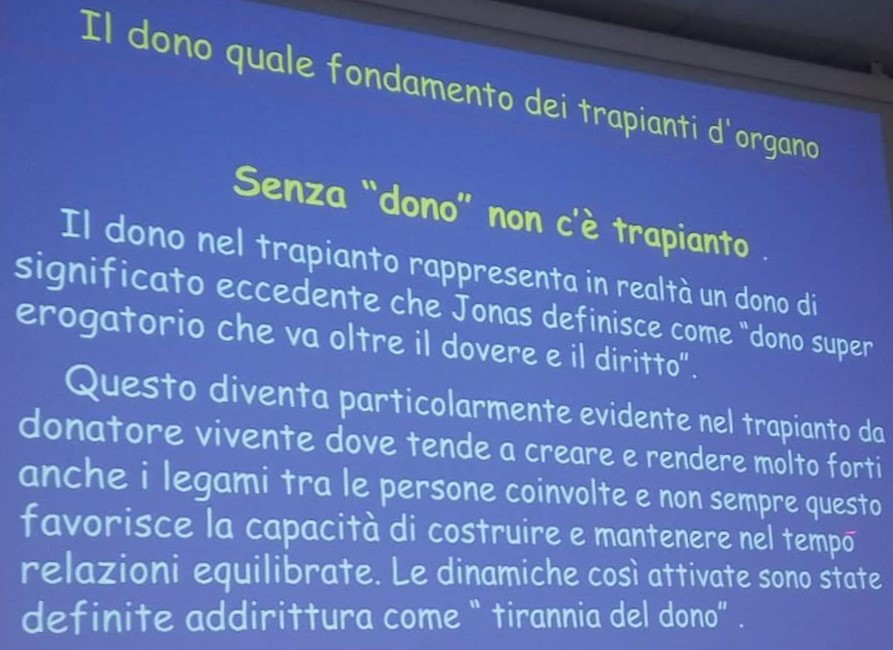
\includegraphics[width=0.7\textwidth]{34/image18.jpeg}
	\end{figure}

``Tirannia del dono'': ci sono purtroppo situazioni in cui per esempio
la mamma obbliga,da un punto di vista psicologico, il fratello a donare
un organo all'altro fratello. Ci sono casi in cui la donazione tra
fratelli non è spontanea, ma c'è un'influenza esterna. È più facile la
donazione tra marito e moglie.

\begin{figure}[!ht]
\centering
	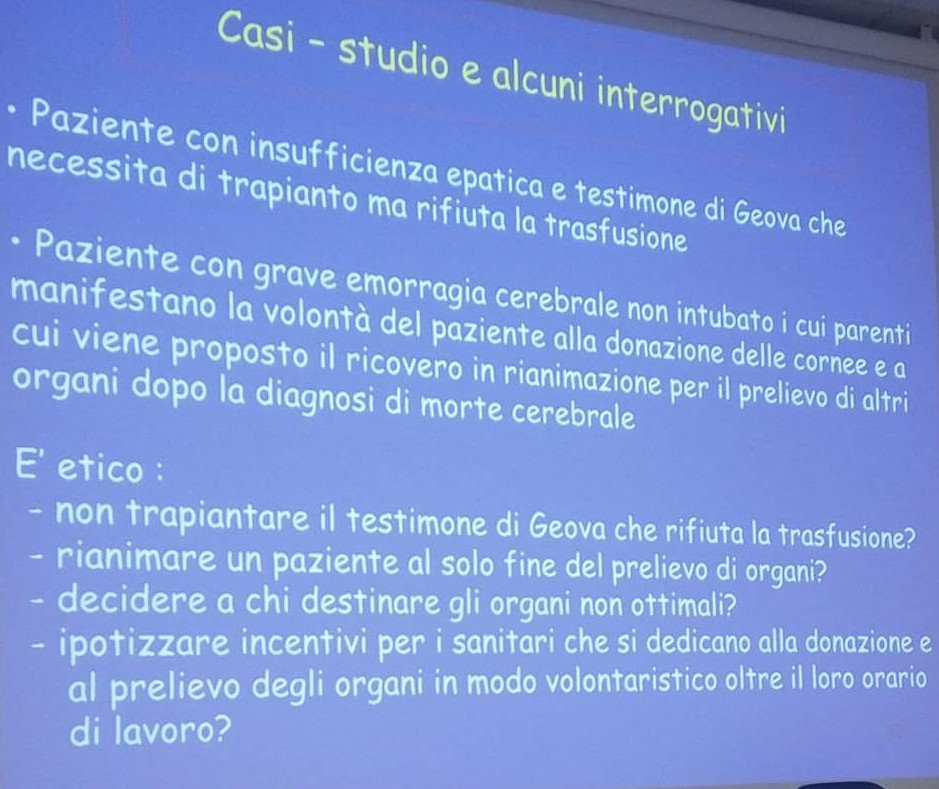
\includegraphics[width=0.7\textwidth]{34/image19.jpeg}
	\end{figure}

Vi lascio con alcuni casi studio e quesiti etici.
\\
In Italia il commercio degli organi non è possibile; i trapianti si
possono fare solo in strutture pubbliche, ma in altre realtà, come ad
esempio in Germania, è possibile fare trapianti pagando il donatore
volontario (non è proprio un commercio, ma è una possibilità; da noi non
si può fare nemmeno questo)
\\
La nostra professione si basa sulla coscienza morale e sulla
responsabilità individuale; il codice diventa una guida insostituibile.
Bisogna dar tempo all'ascolto, parlare al malato, dare importanza al
linguaggio non verbale del malato, e soprattutto curare la speranza
oltre alla malattia.
\subsection{CCEPS: Commissione Centrale per gli Esercenti le Professioni Sanitarie}

È una commissione giurisdizionale, infatti il presidente di Commissione
è un consigliere di Stato, un magistrato. Le sentenze vengono fatte in
nome del popolo italiano. Questa commissione giudica ciò che un
presidente provinciale (come Muzzetto) fa sui suoi iscritti. Se per
esempio il Presidente Muzzetto da una sanzione ad un collega e quel
collega ritiene di essere stato ingiustamente sanzionato, viene in
Commissione Centrale a fare ricorso.
\\
Essa è costituita da un Consigliere di Stato nella veste di Presidente,
da un membro designato dal Consiglio Superiore di Sanità e da 10 membri,
5 effettivi e 5 supplenti designati dalla Federazione Nazionale degli
Ordini e Collegi professionali.. Ogni professione sanitaria (infermieri,
ostetriche..) ha i propri rappresentanti. E poi c'è un segretario
amministrativo.
\\
Le spese sono a carico di tutte le Federazioni Nazionali.
\begin{figure}[!ht]
\centering
	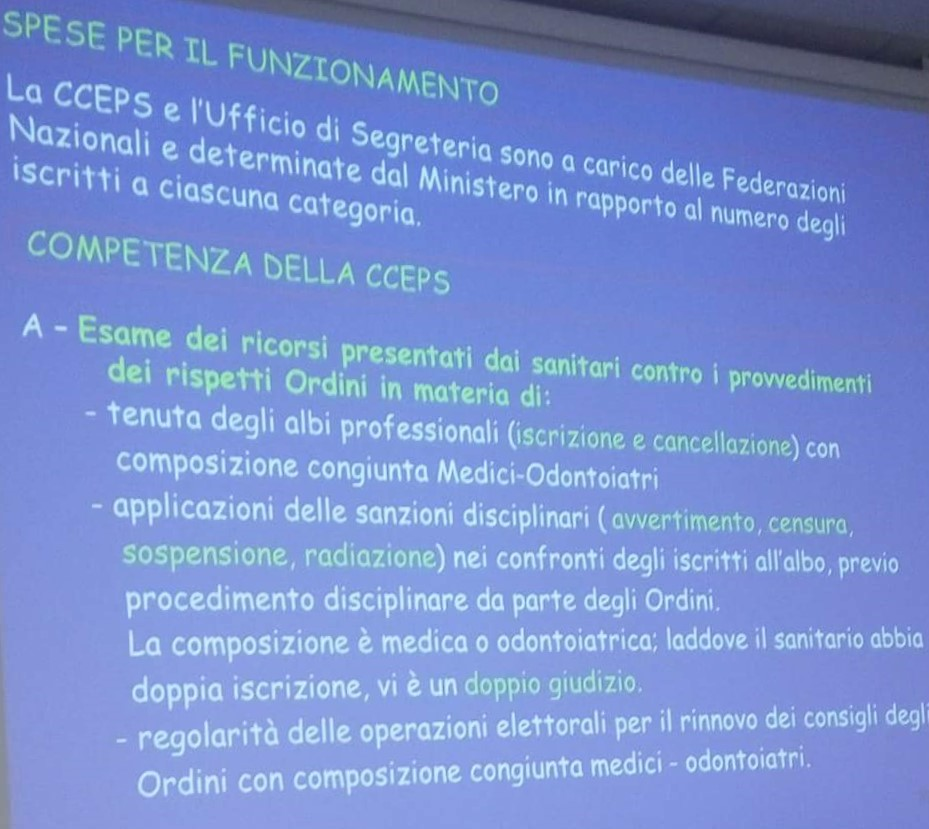
\includegraphics[width=0.7\textwidth]{34/image20.jpeg}
	\end{figure}

I legittimati a proporre ricorso sono: l'iscritto che ha la sanzione
dall'Ordine provinciale, il Ministero della Salute, il Procuratore della
Repubblica e gli stessi Ordini per la difesa della categoria della quale
hanno rappresentanza. Il ricorso deve avvenire entro 30 gg dal
perfezionamento dell'ultima notifica presso la segreteria.
\\
Se il collega viene sospeso e fa ricorso alla CCEPS, questo determina la
sospensione del provvedimento dell'Ordine provinciale (il collega
riprende a lavorare ma viene mantenuto in piedi il provvedimento
disciplinare).
\\
L'Udienza è pubblica; il collega si presenta con un avvocato e viene
ascoltato; viene poi ascoltato l'Ordine (anch'esso con il proprio
avvocato); ci si riunisce in Camera di Consiglio e infine si può o
confermare o ridurre o cancellare il provvedimento dell'Ordine. Non si
può invece aumentare la pena.
\begin{figure}[!ht]
\centering
	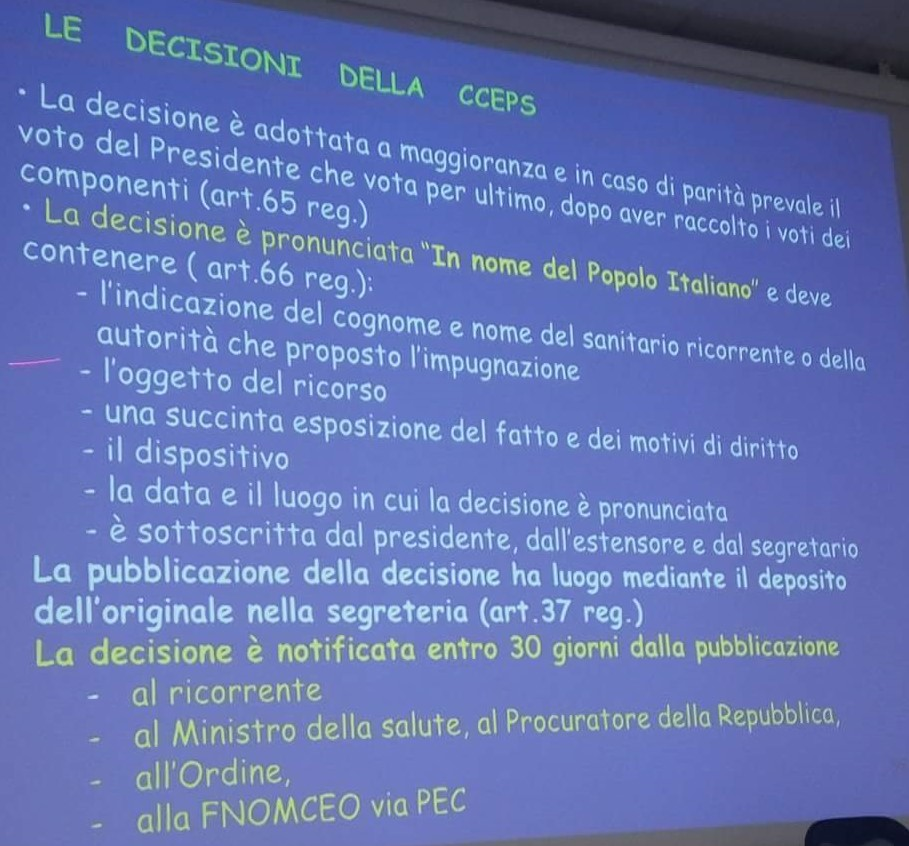
\includegraphics[width=0.7\textwidth]{34/image21.jpeg}
	\end{figure}

Il collega si può poi rivolgere alla Cassazione che può annullare la
sentenza della CCEPS.


